\documentclass[a4paper,titlepage]{article}
\usepackage[top=1in, bottom=1.25in, left=1.25in, right=1.25in]{geometry}

\parskip=10pt

\usepackage[scaled]{beramono}
\usepackage[T1]{fontenc}

\usepackage{amsmath}

\usepackage{listings}
\lstset{
	basicstyle=\footnotesize\ttfamily,
	tabsize=4,
	breaklines,
	frame=single,
	moredelim=[is][\underbar]{__}{__}
}

\usepackage{graphicx}
\usepackage{tikz}
\usepackage{float}
\usepackage{booktabs}

\renewcommand{\figurename}{Gambar}
\renewcommand{\refname}{Referensi}

\begin{document}

	\title{Laporan Tugas Besar 1 \\ IF2121 Logika Informatika \\ - \\ \large K-01 - Kelompok DuniaTidakAdil}
	\author{
			Jonathan Christopher \\
			(13515001)
		\and
			Jordhy Fernando \\
			(13515004)
		\and
			Jauhar Arifin \\
			(13515049)
		\and
			Turfa Auliarachman \\
			(13515133)
	}
	\maketitle

	\section{Deskripsi Program}

		Program yang kelompok kami (DuniaTidakAdil) buat untuk Tugas Besar I mata kuliah Logika Informatika ini bernama \textit{Submerged}. \textit{Submerged} adalah sebuah game petualangan berbasis teks yang diimplementasikan menggunakan bahasa pemrograman deklaratif Prolog. Dalam game ini, pemain harus mengeksplorasi sebuah kapal selam yang sedang tenggelam dan mencari jalan keluar ke permukaan. Pemain dapat melakukan perintah-perintah untuk berpindah tempat, mengambil dan menggunakan objek, serta berinteraksi dengan NPC.

	\section{Keunikan dan Kelebihan}

		Game \textit{Submerged} ini memiliki beberapa keunikan dan kelebihan:

		\begin{itemize}
			\item Game dikompilasi dari program Prolog menjadi sebuah file \textit{executable} yang sudah memuat \textit{interpreter} Prolog, sehingga game dapat langsung dijalankan tanpa terlebih dahulu menjalankan \textit{interpreter} Prolog secara manual.
			\item Meskipun hanya ada 10 ruangan yang dapat didatangi pemain (karena cerita bertempat pada sebuah kapal selam yang sempit), ada banyak kondisi yang harus dipenuhi pemain. Contohnya, untuk membuka pintu ke ruangan-ruangan tertentu, pemain harus sudah menyalakan listrik, lalu membuka pintu melalui panel kendali di ruangan lainnya. Dengan begitu, permainan menjadi tidak terlalu mudah.
			\item Terdapat berbagai nilai yang bersifat seperti \textit{timer} untuk memaksa pemain berusaha menyelesaikan permainan dengan lebih cepat, misalnya jarak kapal musuh, tingkat oksigen, kedalaman, dsb. Nilai-nilai tersebut akan terus berkurang setiap kali pemain pergi ke ruangan lain atau melakukan sebuah aksi. Jika melewati batas tertentu, maka pemain dianggap kalah.
			\item Cerita permainan dibuat dalam bahasa Inggris.
		\end{itemize}

	\section{Peta Permainan dan Daftar Objek}

		\subsection{Peta Permainan}

			\begin{lstlisting}

			                 Airlock                                 Surface
			                    |                                       |
			                    |                                       |
			Weapons room - Sonar room - Control room - Engine room - Reactor
			                    |
			                    |
			Wardroom - Crew's quarters - Storage room


 << Depan  Belakang >>

			\end{lstlisting}

		\subsection{Daftar Objek}

			\noindent Terdapat objek-objek statis maupun interaktif yang terletak pada beberapa lokasi dalam game ini:

			\subsubsection{\textit{Weapons room}}
			\begin{itemize}
				\item \textit{Barrels}: pada awalnya menghalangi pintu keluar, bisa dipindahkan.
				\item \textit{Explosives}: (statis) dapat diaktifkan untuk menghancurkan kapal selam (objektif sekunder), membutuhkan kode pengaktifan yang dapat dilihat di \textit{document} 2.
				\item \textit{Weapons}: (statis) tidak dapat digunakan.
			\end{itemize}

			\subsubsection{\textit{Sonar room}}
			\begin{itemize}
				\item \textit{Sonar display}: (statis) dapat menunjukkan jarak ke kapal musuh (jika terlalu dekat, maka pemain kalah; kecuali jika sudah mengaktifkan \textit{Active Defense System}). Membutuhkan listrik untuk menyala.
				\item \textit{Headphones}: tidak dapat digunakan.
			\end{itemize}

			\subsubsection{\textit{Crew's quarters}}
			\begin{itemize}
				\item \textit{Book, canned food, bucket}: tidak dapat digunakan.
				\item \textit{Knife}: dapat digunakan untuk bunuh diri (menyerah).
			\end{itemize}

			\subsubsection{\textit{Wardroom}}
			\begin{itemize}
				\item \textit{Document 1}: mengandung informasi tentang kapal selam.
				\item \textit{Document 2}: mengandung kode pengaktifan \textit{explosives} yang dapat digunakan untuk menyelesaikan objektif sekunder.
				\item \textit{Document 3}: mengandung kode aktivasi untuk \textit{Active Defense System}.
				\item \textit{Sub's logs}: mengandung cerita.
			\end{itemize}

			\subsubsection{\textit{Storage room}}
			\begin{itemize}
				\item \textit{Diving equipment}: harus dipakai untuk dapat bertahan hidup jika ruangan terisi air (misalnya jika membuka pintu ke ruangan yang berisi air).
				\item \textit{Oxygen canister}: menambah tingkat oksigen sebesar 5 satuan.
				\item \textit{Crowbar}: dapat dipakai memperbesar lubang/menyingkirkan halangan di \textit{Reactor} supaya dapat dilewati untuk keluar.
			\end{itemize}

			\subsubsection{\textit{Control room}}
			\begin{itemize}
				\item \textit{Control panel}: (NPC, statis) dapat berinteraksi untuk mengaktifkan \textit{Active Defense System}, serta \textit{lock/unlock} pintu antar ruangan. Membutuhkan listrik untuk menyala.
				\item \textit{Map}: (statis) menampilkan denah ruangan.
				\item \textit{Radio}: (NPC, statis) dapat berinteraksi untuk mengetahui objektif sekunder (mengaktifkan \textit{explosives}). Membutuhkan listrik untuk menyala.
				\item \textit{Periscope}: (statis) tidak dapat digunakan.
			\end{itemize}

			\subsubsection{\textit{Engine room}}
			\begin{itemize}
				\item \textit{Fuse box}: (statis) dapat berinteraksi untuk menyalakan tenaga listrik cadangan.
				\item \textit{Reactor status display}: (statis) menampilkan informasi bahwa ruang \textit{Reactor} berisi air.
				\item \textit{Fire extinguisher}: perangkap, mengurangi tingkat oksigen sebanyak 3 satuan jika dipakai.
				\item \textit{Oxygen canister}: menambah tingkat oksigen sebanyak 5 satuan jika dipakai.
				\item{Engine spare parts}: tidak dapat digunakan.
			\end{itemize}

			\subsubsection{\textit{Reactor}}
			\begin{itemize}
				\item \textit{Hole}: (statis) lubang pada dinding luar kapal selam; pada awalnya terlalu kecil dan tidak dapat dilewati, tetapi dapat diperbesar menggunakan \textit{crowbar}.
				\item \textit{Engine, dead engineer}: (statis) tidak dapat digunakan.
			\end{itemize}

	\section{Penjelasan \textit{Command}}

		\noindent Terdapat beberapa \textit{command} yang dapat digunakan oleh pemain dalam game ini:

		\begin{itemize}
			\item n/s/e/w: pindah ke ruangan di atas/bawah/kanan/kiri ruangan saat ini.
			\item take(Object): mengambil sebuah objek tidak statis yang terdapat di ruangan tempat pemain berada dan memasukkannya ke dalam \textit{inventory}. Dapat digunakan misalnya ketika berada di \textit{storage room}, dan ingin memasukkan \textit{crowbar} ke dalam \textit{inventory}.
			\item drop(Object): mengeluarkan objek dari \textit{inventory} pemain dan meletakkannya di ruangan tempat pemain berada saat ini.
			\item use(Object): menggunakan sebuah objek yang sedang dibawa dalam \textit{inventory}. Contohnya, menggunakan sebuah \textit{oxygen canister} akan menambah tingkat oksigen sebesar 5 satuan.
			\item move(Object): memindahkan objek yang menghalangi jalan. Misalnya memindahkan \textit{barrels} yang menghalangi pintu di \textit{weapons room}.
			\item switch{Object}: menyalakan/mematikan sebuah saklar. Misalnya menyalakan/mematikan sumber listrik cadangan di \textit{engine room}.
			\item operate(Object): mengoperasikan suatu objek statis, misalnya \textit{control panel} di \textit{control room}.
			\item check: melihat sebuah tampilan status, misalnya melihat keadaan \textit{reactor status display} di \textit{engine room}.
			\item suicide: bunuh diri - jika dilakukan, maka pemain kalah dan permainan berakhir.
			\item talk: untuk berbicara kepada sebuah objek/NPC, contohnya berbicara ke radio di \textit{control room}.
			\item stat: untuk melihat keadaan status dan isi \textit{inventory}.
			\item look: untuk menampilkan ulang keadaan ruangan.
			\item instructions: untuk menampilkan daftar \textit{command}.
			\item save(Filename): untuk menyimpan keadaan pemain dalam sebuah \textit{save file} sesuai parameter \textit{Filename}.
			\item quit: keluar dari permainan.

		\end{itemize}

	\section{Hasil Eksekusi}

		\begin{figure}[h]
		    \centering
		    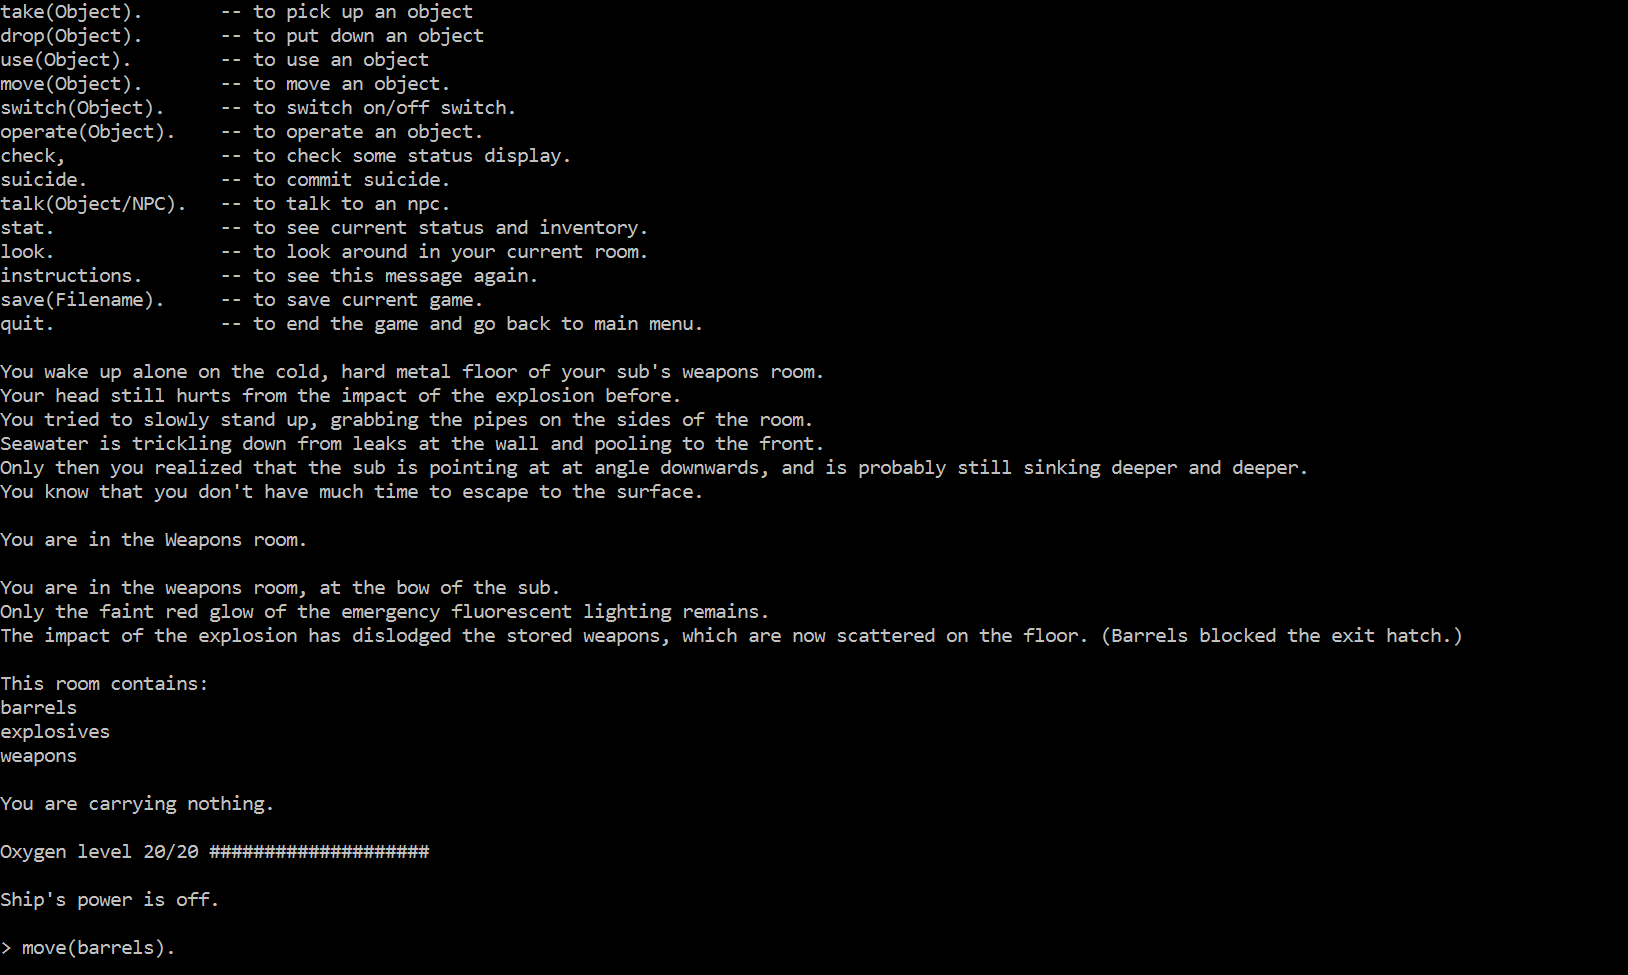
\includegraphics[width=0.5\textwidth]{demo.PNG}
		    \caption{Contoh screenshot hasil eksekusi program}
		    \label{fig:hasileksekusi}
		\end{figure}

		\lstinputlisting{./demo.txt}

	\section{Pembagian Kerja}

		\noindent Berikut adalah tabel pembagian tugas dalam kelompok:

		\begin{table}[H]
			\centering
			\begin{tabular}{@{}lll@{}}
				\toprule
				Komponen & Anggota & Dikerjakan pada \\ \midrule
				\textit{Main loop} dan \textit{menu} & Jonathan & 17 November 2016 \\
				\textit{Makefile} & Jonathan & 16 November 2016 \\
				Teks cerita & Jonathan & 16-29 November 2016 \\
				Laporan & Jonathan & 29 November 2016 \\
				\textit{Load/save} & Jordhy & 28-29 November 2016 \\
				Pindah ruangan & Jauhar, Jordhy & 23-24 November 2016 \\
				\textit{Oxygen level} & Turfa & 24 November 2016 \\
				\textit{Take/drop} & Jordhy & 24 November 2016 \\
				\textit{Check, talk, suicide} & Jauhar & 29 November 2016 \\
				\textit{Operate, look, stat, instructions} & Jordhy & 29 November 2016 \\
				\textit{Win/lose} & Jordhy & 29 November 2016 \\
				\textit{Game states + getter/setter} & Turfa & 24-29 November 2016 \\
				\textit{Active defense system AI} & Jauhar & 29 November 2016 \\
				\textit{Tests} & Jauhar & 29 November 2016 \\
			\end{tabular}
		\end{table}

\end{document}
